\section{Unterstützungs-App (JH)}
Die Unterstützungs-App soll die Hauptanwendung um die Möglichkeit erweitern, Ausleihen und Rückgaben durch Unterstützer direkt in den Klassen durchzuführen. Zu diesem Zweck wurde eine App entwickelt, welche die genannten Funktionen bietet und (derzeit) auf einem Android-Smartphone installiert werden kann.
\subsection{Datenübertragung per Ad-Hoc Verbindung}
Um Zugriff auf die Daten der LibOrg-Anwendung zu bekommen, war ursprünglich ein Ad-Hoc-Netzwerkverbindung zwischen dem Rechner, auf dem die Hauptanwendung läuft, und der App auf einem Android-Smartphone geplant. Leider unterstützt Android Ad-Hoc-Netzwerke jedoch unerwarteterweise nicht. Aus diesem Grund musste auf die Hotspot-Technologie zurückgegriffen werden. Hierbei muss zuerst der Hotspot auf dem Android Gerät aktiviert werden und dann der Rechner, auf dem die Hauptanwendung läuft, auf diesen verbunden werden. Dies ist für den Kunden zu aufwendig, deshalb kann alternativ das Smartphone und der Laptop mit dem gleichen Access Point verbunden werden. Daraufhin muss im Hauptprogramm die Unterstützungsfunktion gestartet werden und die dort angezeigte IP-Adresse und der Port in der App eingetragen werden. Anschließend kann man Verbinden und dann von der Hauptanwendung die Datenbank an das Smartphone übertragen. Danach kann die Klassenauswahl erfolgen.
\begin{figure}[H]
	\centering
		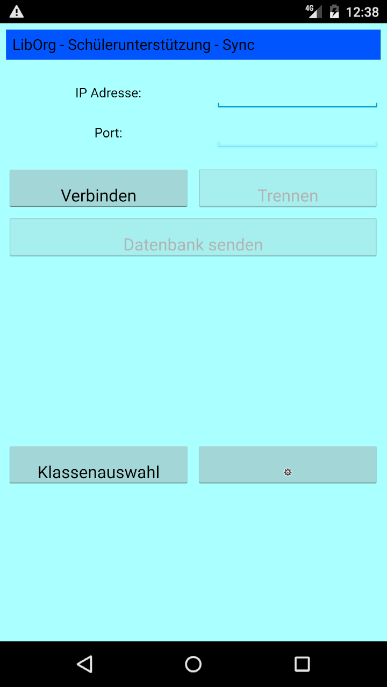
\includegraphics[width=0.30\textwidth]{figures/SupportApp/Verbindung.png}
	\caption{Verbindungsansicht der Support-App}
	\label{fig:Verbindungsansicht App}
\end{figure}

\subsection{Klassen und Schülerauswahl}
Die folgenden Dialoge bieten die Möglichkeit zuerst eine Klasse und dann einen Schüler auszuwählen. Allerdings können die Bücher auch klassenweise ausgeliehen und zurückgegeben werden.
\begin{figure}[H]
	\centering
		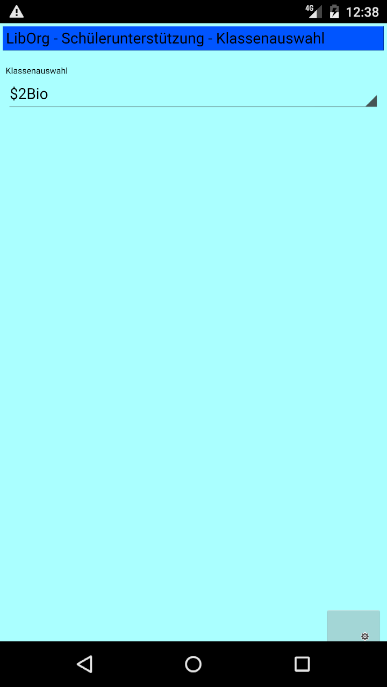
\includegraphics[width=0.30\textwidth]{figures/SupportApp/Klassenauswahl.png}
	\caption{Klassenauswahl der Support-App}
	\label{fig:Klassenauswahl App}
\end{figure}

\begin{figure}[H]
	\centering
		\includegraphics[width=0.30\textwidth]{figures/SupportApp/Schülerauswahl.png}
	\caption{Schülerauswahl der Support-App}
	\label{fig:Schülerauswahl App}
\end{figure}

\subsection{Ausleihe und Rückgabe von Büchern}
Zuletzt kommt man zur eigentlichen Funktion der App, das Ausleihen und Zurückgeben. Je nach Auswahl entweder pro Schüler oder klassenweise. Wichtig ist hierbei, dass bei der klassenweisen Rückgabe von Büchern sicher gestellt werden muss, dass kein Buch Beschädigungen aufweist, da die Überprüfung auf Schäden nur bei der Einzelrückgabe erfolgt.
\begin{figure}[H]
	\centering
		\includegraphics[width=0.30\textwidth]{figures/SupportApp/Schülerausleihe.png}
	\caption{Schülerausleihe der Support-App}
	\label{fig:Schülerausleihe App}
\end{figure}

\begin{figure}[H]
	\centering
		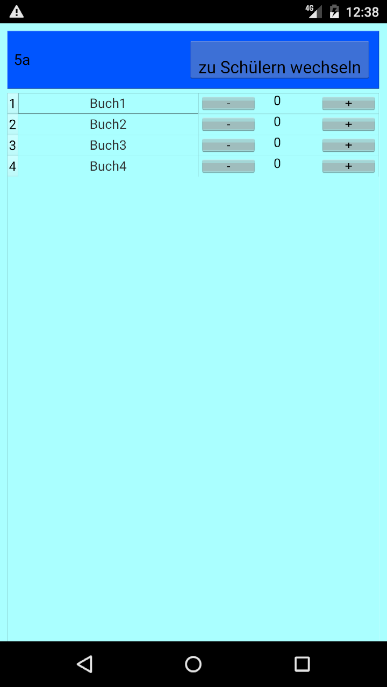
\includegraphics[width=0.30\textwidth]{figures/SupportApp/Klassenausleihe.png}
	\caption{Klassenausleihe der Support-App}
	\label{fig:Klassenausleihe App}
\end{figure}

Die App stellt eine erste Version mit den wichtigsten Funktionen dar und kann in Zukunft noch um einige Funktionalitäten erweitert werden. So kann zum Beispiel eine Abfrage der Beschädigungen in der klassenweisen Rückgabe erfolgen oder eine Ferienausleihe einzelner Bücher erfolgen. Ebenfalls kann noch vieles an der Usability und am Overlay angepasst werden. Des Weiteren könnte man mehrere Android- Geräte mit unterschiedlichen Datenbeständen losschicken und diese zum Schluss in der Hauptanwendung wieder zusammenführen. Dafür wären allerdings Änderungen in der Hauptanwendung und ein ausgeklügeltes Übertragungsprotokoll notwendig.